\chapter{Methods}
\label{ch:methods}

\section{DQN Implementation}
\label{sec:dqn-implementation}

\subsection{Input Preprocessing}
\label{subsec:input-preprocessing}

\vspace{2em}

\subsection{Network Architecture}
\label{subsec:network-architecture}

\begin{figure}[ht]
\centering
\definecolor{convfront}{HTML}{B8CCE4}
\definecolor{convtop}{HTML}{D0DEF0}
\definecolor{convside}{HTML}{8FAEC8}
\definecolor{fcfront}{HTML}{C5D5C5}
\definecolor{fctop}{HTML}{D8E6D8}
\definecolor{fcside}{HTML}{9AB89A}
\definecolor{outfront}{HTML}{D4C5B0}
\definecolor{outtop}{HTML}{E4D8C8}
\definecolor{outside}{HTML}{B8A890}
\resizebox{0.85\textwidth}{!}{%
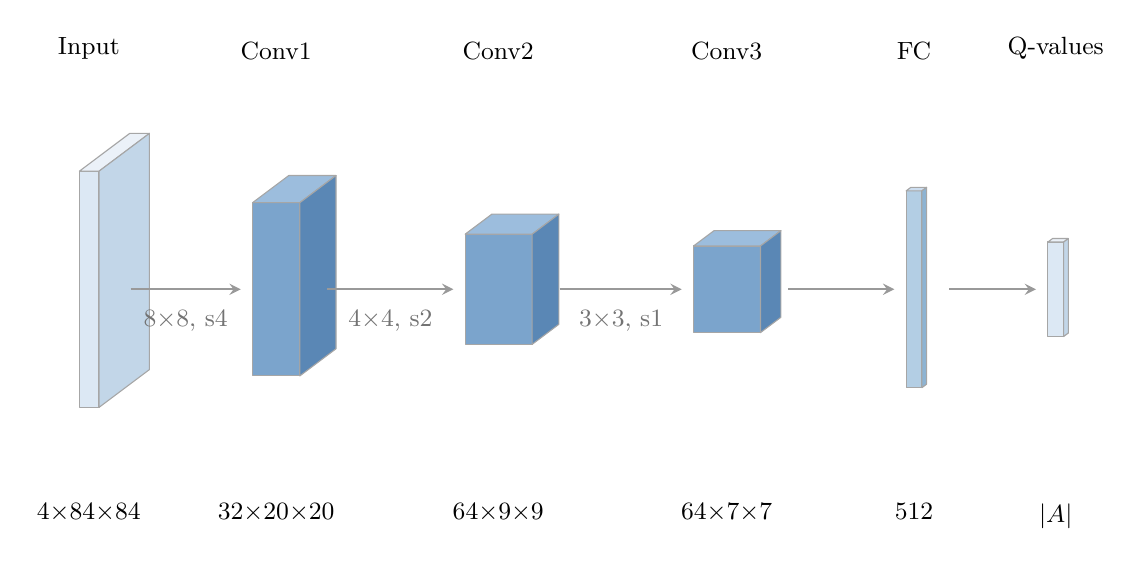
\begin{tikzpicture}[
    x={(1cm,0cm)}, y={(0cm,1cm)}, z={(0.4cm,0.3cm)},
    arr/.style={->, thick, >=stealth, black!40},
    dimlbl/.style={font=\small, anchor=north},
    namelbl/.style={font=\small, anchor=south},
    filtlbl/.style={font=\small, text=black!55, anchor=north}
]

\newcommand{\cuboid}[7]{
    \fill[#5, draw=black!35, line join=round]
        (#1, {-#3/2}, 0) -- ({#1+#2}, {-#3/2}, 0) --
        ({#1+#2}, {#3/2}, 0) -- (#1, {#3/2}, 0) -- cycle;
    \fill[#6, draw=black!35, line join=round]
        (#1, {#3/2}, 0) -- ({#1+#2}, {#3/2}, 0) --
        ({#1+#2}, {#3/2}, #4) -- (#1, {#3/2}, #4) -- cycle;
    \fill[#7, draw=black!35, line join=round]
        ({#1+#2}, {-#3/2}, 0) -- ({#1+#2}, {#3/2}, 0) --
        ({#1+#2}, {#3/2}, #4) -- ({#1+#2}, {-#3/2}, #4) -- cycle;
}

% Baselines
\def\dimY{-2.6}
\def\nameY{2.8}

% Input: 4 x 84 x 84
\cuboid{0.8}{0.25}{3.0}{1.6}{outfront}{outtop}{outside}
\node[namelbl] at (0.92, \nameY, 0) {Input};
\node[dimlbl] at (0.92, \dimY, 0) {4${\times}$84${\times}$84};

% Arrow + label below
\draw[arr] (1.45, 0, 0) -- (2.85, 0, 0);
\node[filtlbl] at (2.15, -0.15, 0) {8${\times}$8, s4};

% Conv1: 32 x 20 x 20
\cuboid{3.0}{0.6}{2.2}{1.15}{convfront}{convtop}{convside}
\node[namelbl] at (3.3, \nameY, 0) {Conv1};
\node[dimlbl] at (3.3, \dimY, 0) {32${\times}$20${\times}$20};

% Arrow + label below
\draw[arr] (3.95, 0, 0) -- (5.55, 0, 0);
\node[filtlbl] at (4.75, -0.15, 0) {4${\times}$4, s2};

% Conv2: 64 x 9 x 9
\cuboid{5.7}{0.85}{1.4}{0.85}{convfront}{convtop}{convside}
\node[namelbl] at (6.12, \nameY, 0) {Conv2};
\node[dimlbl] at (6.12, \dimY, 0) {64${\times}$9${\times}$9};

% Arrow + label below
\draw[arr] (6.9, 0, 0) -- (8.45, 0, 0);
\node[filtlbl] at (7.68, -0.15, 0) {3${\times}$3, s1};

% Conv3: 64 x 7 x 7
\cuboid{8.6}{0.85}{1.1}{0.65}{convfront}{convtop}{convside}
\node[namelbl] at (9.02, \nameY, 0) {Conv3};
\node[dimlbl] at (9.02, \dimY, 0) {64${\times}$7${\times}$7};

% Arrow
\draw[arr] (9.8, 0, 0) -- (11.15, 0, 0);

% FC: 512
\cuboid{11.3}{0.2}{2.5}{0.15}{fcfront}{fctop}{fcside}
\node[namelbl] at (11.4, \nameY, 0) {FC};
\node[dimlbl] at (11.4, \dimY, 0) {512};

% Arrow
\draw[arr] (11.85, 0, 0) -- (12.95, 0, 0);

% Q-values
\cuboid{13.1}{0.2}{1.2}{0.15}{outfront}{outtop}{outside}
\node[namelbl] at (13.2, \nameY, 0) {Q-values};
\node[dimlbl] at (13.2, \dimY, 0) {$|A|$};

\end{tikzpicture}%
}
\caption{Nature CNN architecture. Block height reflects spatial
  dimensions; block depth reflects channel count. All convolutional
  and fully connected layers use ReLU activation.}
\label{fig:nature-cnn}
\end{figure}


\begin{table}[ht]
\centering
\renewcommand{\arraystretch}{1.4}
\begin{tabular}{llcccc}
\toprule
Layer & Type & Filters & Kernel & Stride & Output \\
\midrule
Input    & --             & --  & --            & --  & $4 \times 84 \times 84$ \\
Conv1    & Conv2d + ReLU  & 32  & $8 \times 8$  & 4   & $32 \times 20 \times 20$ \\
Conv2    & Conv2d + ReLU  & 64  & $4 \times 4$  & 2   & $64 \times 9 \times 9$ \\
Conv3    & Conv2d + ReLU  & 64  & $3 \times 3$  & 1   & $64 \times 7 \times 7$ \\
Flatten  & --             & --  & --            & --  & 3136 \\
FC       & Linear + ReLU  & --  & --            & --  & 512 \\
Q-head   & Linear         & --  & --            & --  & $|A|$ \\
\bottomrule
\end{tabular}
\caption{Nature CNN layer specifications. Each convolutional layer
  applies the listed kernel with the given stride, followed by ReLU
  activation. The output layer is linear.}
\label{tab:nature-cnn-layers}
\end{table}


\vspace{2em}

\subsection{Training Procedure}
\label{subsec:training-procedure}

\vspace{2em}

\subsection{Experience Replay}
\label{subsec:experience-replay}

\vspace{2em}

\subsection{Target Network}
\label{subsec:target-network}

\vspace{2em}

\subsection{Atari-100K Adaptations}
\label{subsec:atari100k-adaptations}

\vspace{4em}

\section{Data Augmentation}
\label{sec:augmentation-method}

\section{Self-Predictive Representations}
\label{sec:spr-architecture}

\section{Experiment Design}
\label{sec:experiment-design}

\section{Interpretability Methods}
\label{sec:interpretability-methods}

\subsection{Linear Probing}
\label{subsec:linear-probing}

To evaluate what information the encoder captures, we use linear
probing~(\cref{fig:linear-probe}). The encoder $f_\theta$ is first
trained end-to-end via reinforcement learning, then its weights are
frozen. A single linear layer is trained on the frozen
representations to predict known game-state properties. Because the
probe is restricted to a linear mapping, any structure it recovers
must already be present in the representation -- the probe cannot
learn new features of its own. Probe accuracy therefore measures
what information $f_\theta$ has made linearly accessible.

\begin{figure}[ht]
\centering
% Reuse Nature CNN colors
\definecolor{convfront}{HTML}{7BA4CC}
\definecolor{convtop}{HTML}{9CBDDD}
\definecolor{convside}{HTML}{5A87B5}
\definecolor{fcfront}{HTML}{B3CEE4}
\definecolor{fctop}{HTML}{CDDEF0}
\definecolor{fcside}{HTML}{8DB3D2}
\definecolor{outfront}{HTML}{DCE8F4}
\definecolor{outtop}{HTML}{EBF1F8}
\definecolor{outside}{HTML}{C2D6E8}
% Probe colors
\definecolor{probeorange}{HTML}{E8B87A}
\definecolor{predorange}{HTML}{F5E0C8}
\definecolor{gtgreen}{HTML}{D4ECD4}
% Faded encoder
\definecolor{encfade}{HTML}{B8D2E6}

%% --- (a) Frozen encoder concept ---
\begin{subfigure}[t]{\textwidth}
\centering
\resizebox{0.92\textwidth}{!}{%
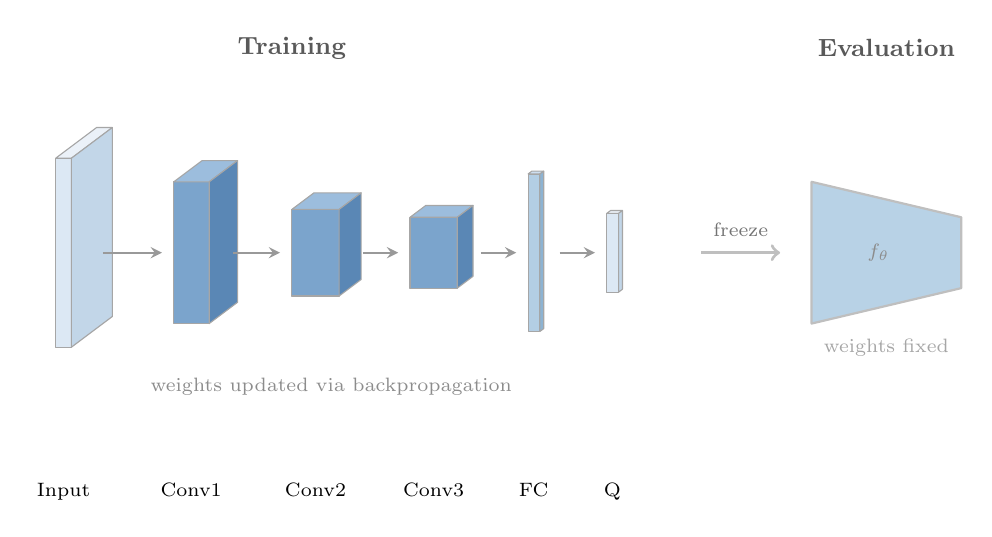
\begin{tikzpicture}[
    x={(1cm,0cm)}, y={(0cm,1cm)}, z={(0.4cm,0.3cm)},
    arr/.style={->, thick, >=stealth, black!40},
    lbl/.style={font=\scriptsize, text=black!55},
    phase/.style={font=\small\bfseries, text=black!65},
    namelbl/.style={font=\scriptsize, anchor=north},
]

\newcommand{\cuboid}[7]{
    \fill[#5, draw=black!35, line join=round]
        (#1, {-#3/2}, 0) -- ({#1+#2}, {-#3/2}, 0) --
        ({#1+#2}, {#3/2}, 0) -- (#1, {#3/2}, 0) -- cycle;
    \fill[#6, draw=black!35, line join=round]
        (#1, {#3/2}, 0) -- ({#1+#2}, {#3/2}, 0) --
        ({#1+#2}, {#3/2}, #4) -- (#1, {#3/2}, #4) -- cycle;
    \fill[#7, draw=black!35, line join=round]
        ({#1+#2}, {-#3/2}, 0) -- ({#1+#2}, {#3/2}, 0) --
        ({#1+#2}, {#3/2}, #4) -- ({#1+#2}, {-#3/2}, #4) -- cycle;
}

\def\dimY{-2.8}

% Phase label
\node[phase] at (3.0, 2.6) {Training};

% Input
\cuboid{0}{0.2}{2.4}{1.3}{outfront}{outtop}{outside}
\node[namelbl] at (0.1, \dimY) {Input};

\draw[arr] (0.6, 0, 0) -- (1.35, 0, 0);

% Conv1
\cuboid{1.5}{0.45}{1.8}{0.9}{convfront}{convtop}{convside}
\node[namelbl] at (1.72, \dimY) {Conv1};

\draw[arr] (2.25, 0, 0) -- (2.85, 0, 0);

% Conv2
\cuboid{3.0}{0.6}{1.1}{0.7}{convfront}{convtop}{convside}
\node[namelbl] at (3.3, \dimY) {Conv2};

\draw[arr] (3.9, 0, 0) -- (4.35, 0, 0);

% Conv3
\cuboid{4.5}{0.6}{0.9}{0.5}{convfront}{convtop}{convside}
\node[namelbl] at (4.8, \dimY) {Conv3};

\draw[arr] (5.4, 0, 0) -- (5.85, 0, 0);

% FC
\cuboid{6.0}{0.15}{2.0}{0.12}{fcfront}{fctop}{fcside}
\node[namelbl] at (6.07, \dimY) {FC};

\draw[arr] (6.4, 0, 0) -- (6.85, 0, 0);

% Q-head
\cuboid{7.0}{0.15}{1.0}{0.12}{outfront}{outtop}{outside}
\node[namelbl] at (7.07, \dimY) {Q};

% Trainable label
\node[font=\scriptsize, text=black!45] at (3.5, -1.7, 0)
    {weights updated via backpropagation};

% --- Freeze arrow ---
\draw[->, very thick, black!25]
    (8.2, 0) -- (9.2, 0)
    node[midway, above=2pt, lbl] {freeze};

% --- Phase 2: Frozen encoder (compact trapezoid) ---
\node[phase] at (10.55, 2.6) {Evaluation};

% Compact encoder trapezoid (no inputs/outputs -- (b) covers that)
\fill[encfade, draw=black!25, thick, line join=round]
    (9.6, -0.9) -- (9.6, 0.9) -- (11.5, 0.45) -- (11.5, -0.45) -- cycle;
\node[font=\scriptsize, text=black!45] at (10.45, 0) {$f_\theta$};

\node[lbl, text=black!35] at (10.55, -1.2) {weights fixed};

\end{tikzpicture}%
}
\caption{The encoder is trained end-to-end via RL, then its weights
  are frozen for linear probing.}
\label{fig:frozen-encoder}
\end{subfigure}

\vspace{1.2em}

%% --- (b) Linear probe concept ---
\begin{subfigure}[t]{\textwidth}
\centering
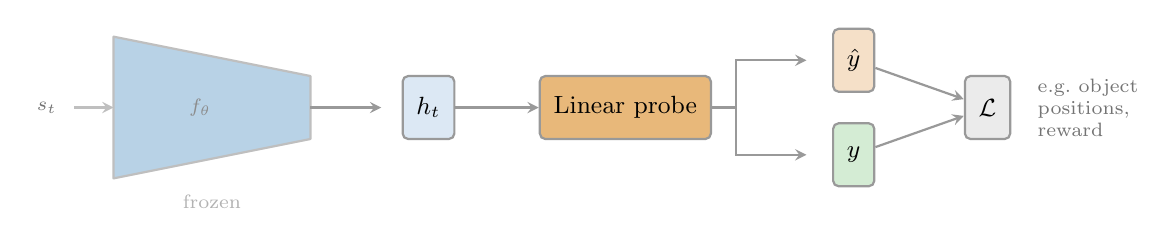
\begin{tikzpicture}[
    box/.style={draw=black!40, thick, minimum height=0.8cm,
                font=\small, inner sep=5pt, rounded corners=2pt},
    arr/.style={->, thick, >=stealth, black!40},
    lbl/.style={font=\scriptsize, text=black!55},
]

% Frozen encoder (trapezoid matching subfigure a)
\node[lbl] at (-0.1, 0) [left] {$s_t$};
\draw[arr, black!25] (0.0, 0) -- (0.5, 0);

\fill[encfade, draw=black!25, thick, line join=round]
    (0.5, -0.9) -- (0.5, 0.9) -- (3.0, 0.4) -- (3.0, -0.4) -- cycle;
\node[font=\scriptsize, text=black!45] at (1.6, 0) {$f_\theta$};
\node[lbl, text=black!30] at (1.75, -1.2) {frozen};

% h_t
\draw[arr] (3.0, 0) -- (3.9, 0);
\node[box, fill=outfront] (repr) at (4.5, 0) {$h_t$};

% Linear probe
\draw[arr] (repr) -- (5.9, 0);
\node[box, fill=probeorange, minimum width=1.6cm] (probe)
    at (7.0, 0) {Linear probe};

% Fork to prediction and ground truth
\draw[arr] (probe.east) -- ++(0.3,0) |- (9.3, 0.6);
\draw[arr] (probe.east) -- ++(0.3,0) |- (9.3, -0.6);

\node[box, fill=predorange] (pred) at (9.9, 0.6) {$\hat{y}$};
\node[box, fill=gtgreen] (gt) at (9.9, -0.6) {$y$};

% Loss
\node[box, fill=black!8, font=\small] (loss) at (11.6, 0)
    {$\mathcal{L}$};
\draw[arr] (pred) -- (loss);
\draw[arr] (gt) -- (loss);

% Annotation
\node[lbl, anchor=west, align=left] at (loss.east) [xshift=6pt]
    {e.g.\ object\\positions,\\reward};

\end{tikzpicture}
\caption{A linear probe is trained on frozen representations to
  predict game-state properties. Probe accuracy measures what
  information $h_t$ contains.}
\label{fig:linear-probe-concept}
\end{subfigure}

\vspace{1.2em}

%% --- (c) Probe attachment points ---
\begin{subfigure}[t]{\textwidth}
\centering
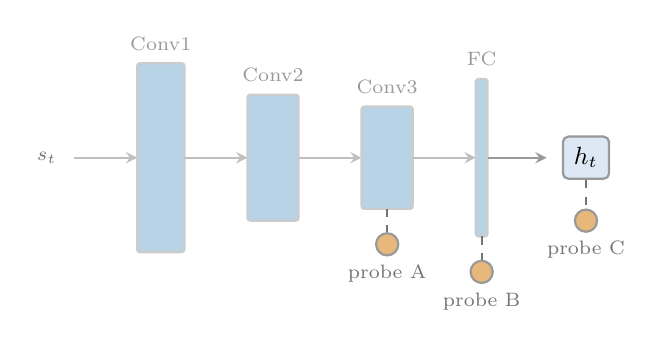
\begin{tikzpicture}[
    arr/.style={->, thick, >=stealth, black!40},
    lbl/.style={font=\scriptsize, text=black!55},
    blklbl/.style={font=\scriptsize, text=black!40},
    probemark/.style={circle, fill=probeorange, draw=black!40,
                      thick, minimum size=8pt, inner sep=0pt},
]

% Input
\node[lbl] at (-0.1, 0) [left] {$s_t$};
\draw[arr, black!25] (0.0, 0) -- (0.8, 0);

% Conv1
\fill[encfade, draw=black!20, thick, rounded corners=1pt]
    (0.8, -1.2) rectangle (1.4, 1.2);
\node[blklbl] at (1.1, 1.45) {Conv1};

\draw[arr, black!25] (1.4, 0) -- (2.2, 0);

% Conv2
\fill[encfade, draw=black!20, thick, rounded corners=1pt]
    (2.2, -0.8) rectangle (2.85, 0.8);
\node[blklbl] at (2.525, 1.05) {Conv2};

\draw[arr, black!25] (2.85, 0) -- (3.65, 0);

% Conv3
\fill[encfade, draw=black!20, thick, rounded corners=1pt]
    (3.65, -0.65) rectangle (4.3, 0.65);
\node[blklbl] at (3.975, 0.9) {Conv3};

\draw[arr, black!25] (4.3, 0) -- (5.1, 0);

% FC
\fill[encfade, draw=black!20, thick, rounded corners=1pt]
    (5.1, -1.0) rectangle (5.25, 1.0);
\node[blklbl] at (5.175, 1.25) {FC};

\draw[arr] (5.25, 0) -- (6.0, 0);

% h_t
\node[draw=black!40, thick, fill=outfront, rounded corners=2pt,
      font=\small, inner sep=4pt] (ht) at (6.5, 0) {$h_t$};

% Probe markers
\node[probemark] (m3) at (3.975, -1.1) {};
\node[probemark] (mfc) at (5.175, -1.45) {};
\node[probemark] (mr) at (6.5, -0.8) {};

\draw[thick, dashed, black!55] (3.975, -0.65) -- (m3);
\draw[thick, dashed, black!55] (5.175, -1.0) -- (mfc);
\draw[thick, dashed, black!55] (ht.south) -- (mr);

\node[lbl] at (m3) [below=4pt] {probe A};
\node[lbl] at (mfc) [below=4pt] {probe B};
\node[lbl] at (mr) [below=4pt] {probe C};

\end{tikzpicture}
\caption{Independent probes at different depths reveal how
  information develops through the network
  (see \cref{fig:nature-cnn} for architecture details).}
\label{fig:linear-probe-layers}
\end{subfigure}

\caption{Linear probe methodology. (a)~The encoder trains via RL and
  is then frozen. (b)~A linear probe predicts game-state properties
  from the frozen encoder's representations. (c)~Probes attached at
  multiple layers measure how information develops across the network.}
\label{fig:linear-probe}
\end{figure}


\indent This approach lets us compare representations across experimental
conditions (e.g., with and without SPR, or across agent
architectures) on a common basis: we hold the probing procedure
fixed and vary only the encoder that produced the representations.
Differences in probe accuracy reflect differences in what the
encoder has learned to represent, not differences in probe capacity.

\subsection{Probe Design}
\label{subsec:probe-design}

Each probe is a single fully connected layer mapping from the
representation $h_t \in \mathbb{R}^d$ to a target
$y \in \mathbb{R}^k$, trained with mean squared error for
continuous targets and cross-entropy for categorical targets. We
train probes on states sampled from completed evaluation episodes,
using the same set of states across all conditions to ensure
comparability.

\smallskip
The probe targets are game-state properties that a capable agent
should represent: object positions, score-relevant features, and
spatial relationships. The specific targets vary by game and are
defined in \cref{sec:experiment-design}. For each target, we report
probe accuracy (classification) or $R^2$ (regression) on a held-out
test set.

\subsection{Probe Attachment Points}
\label{subsec:probe-attachment}

We attach independent probes at multiple points in the encoder to
understand how information develops through the network
(\cref{fig:linear-probe-layers}). Specifically, we probe after
Conv3, after the fully connected layer, and at the final
representation $h_t$. Each probe is trained separately with its own
linear layer.

\smallskip
Probing at multiple depths reveals whether information is present
early (in spatial feature maps) or only emerges after compression
into the fully connected layers. This is informative for
understanding how SPR and data augmentation reshape the encoder's
internal representations, not just its final output.
